\documentclass[spanish]{article}
\usepackage[spanish]{babel}
\usepackage{amsmath}
\usepackage{amssymb}
\usepackage[utf8]{inputenc}
\usepackage{vmargin}
\usepackage{graphicx}
\usepackage{wrapfig}
\usepackage[export]{adjustbox}


\begin{document}
\setpapersize{USletter}
	\setmarginsrb{30mm}{30mm}{30mm}{30mm}{0pt}{0mm}{0pt}{0mm}
	\begin{center}
	{\Large Análisis de Algoritmos, Sem: 2018-1, 3CV2 Práctica 5, 12 de Octubre del 2017}\\
	{\huge {\bf Práctica 5: Algoritmo de Strassen}} \\
	{\large {\bf Luis Daniel Martinez Berumen}}\\
	
\includegraphics[width=1\textwidth]{./imagenes/logos.png}\\
\end{center}
	
	\bigskip
	
	\bigskip
	
	\bigskip
	
	{\LARGE {\bf Abstract}}\\
En esta practica vamos a demostrar la complejidad del algoritmo de Strassen, un algortimo de multiplicacion de matrices que se basa en la descomposicion en simples sumas, llevando acabo el analisis de manera grafica, nos ayudaremos sabiendo que el resultado a obtener es: $O(n^{2.8})$, como lo vimos en clase.\\
Se realizara de igual manera en analisis de el procedimiento normal para multiplicacion de matrices, cabe señalar que las matrices que utilizaremos para estos procesos son cuadradas con orden $2^{n}$
\bigskip
	{\Large {\bf Palabras Clave}}\\
	\begin{itemize}
		\item Algoritmo
		\item Fucion
		\item Recursividad
		\item Orden
		\item Matriz
	\end{itemize}
	
	\section{Introducci\'on}
	Divide y Vencerás es una frase quye hemos escuchado todos, al menos, una vez en nuestra vida, para nosotros 
	es técnica de diseño de algoritmos, siendo de gran utilidad para nuestra carrera, ya que, 
	los problemas a los que nos enfrentamos día con día son mas faciles de resolver si aplciamos una tecnica de este tipo.
	De hecho, suele ser considerada una filosofía general para resolver problemas, no solo del termino informatico, sino que también           se utiliza en muchos otros ámbitos

\newpage
	\section{Conceptos B\'asicos}
	Para la correcta comprension de este trabajo, es necesario definir algunos terminos tales como $\theta$, O y $\Omega$.\\
	 $\theta$(n):\\
		Sea g(n) una función. Se define  $\theta$ (g(n)) como:\\
		
		 	$\theta$(g(n)) = $\{ f(n) \quad | \quad \exists c1,c2>0 \quad \& \quad n_{0}>0 \quad \mid \quad \forall n>=n_{0} \quad 0<= c1g(n) <= f(n) <= c2g(n) \}$
	\bigskip		 	
		 	
	O(n):\\
		Sea  g(n)  una función, O(n) (el pero de los casos) se define como:\\
		
			\hspace{1cm}O(n)=$\{f(n) \quad | \quad \exists c >0 \quad \& \quad n_{0}>0 \quad | \quad f(n) <= Cg(n) \quad \forall  n>= n_{0} \}$
	\bigskip
	
	$\Omega$(n):\\
	Sea  g(n)  una función. Se define $\Omega$ (g(n)) (el mejor de los casos) como:\\

		\hspace{1cm}$\Omega$(g(n)) =$\{f(n) \quad | \quad \exists c >0 \quad \& \quad n_{0}>0 \quad \mid \quad  0<= cg(n)<= f(n) \quad \forall n>= n_{0} \}$
	\bigskip

	\begin{center}
		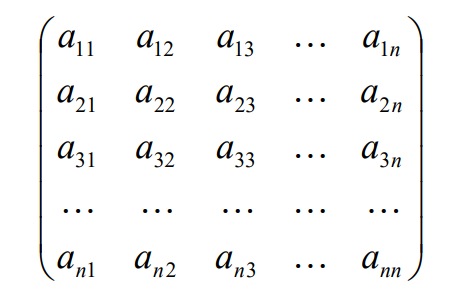
\includegraphics[width=100mm]{./imagenes/figuno.png}\\
		Figura 1: Matriz Cuadrada
	\end{center}
	Para la correcta comprension de esta practica, debemos definir el concepto de una matriz cuadrada, siendo esta una matriz que 		tiene tantas filas como columnas, como podemos apreciar en la figura 1, la matriz se compone de mxn elementos, en el caso de 		una matriz cuadrada, se restringe esta propiedad al tener que ser m=n, por lo tanto la matriz quedara como de nxn elementos.
\newpage
Tomando como ejemplo una amtriz caudrada de orden 2, ejemplificaremos el uso del algoritmo de Strassen:

	\begin{center}
		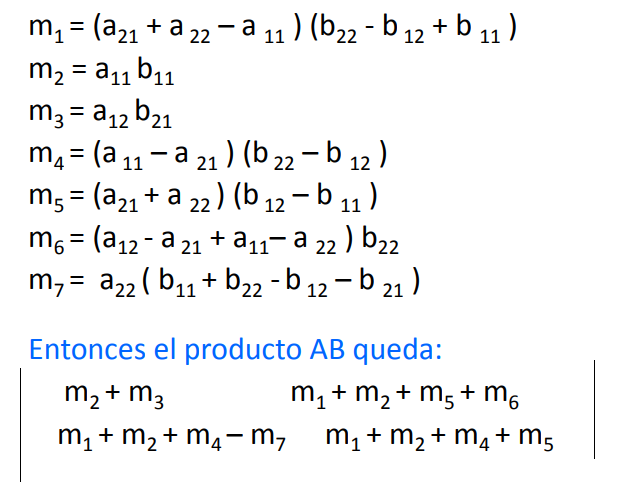
\includegraphics[width=100mm]{./imagenes/fig3.png}\\
		Figura 2: Operaciones Resultantes
	\end{center}
	
	\bigskip
	
	Si reemplazamos cada elemento de A y B por una matriz de n x n, las fórmulas anteriores nos dan una forma de multiplicar dos 2n X 2n matrices.
	A partir de esto tenemos un método recursivo para calcular el producto de matrices con n Algoritmo de multiplicación de Strassen potencia de 2.
	Este método se puede generalizar también a matrices cuyas dimensiones no sean de la forma 2n 	

	\newpage	

	\section{Experimentaci\'on y Resultados}
	
	\subsection{Implemente el algortimo Stressen para producto de matrices.}
	
	{\large i)Mediante graficas, muestre que el algoritmo de {\bf Strassen} tiene complejidad $O(n^{2.8})$.}\\

	\bigskip

	\begin{center}
		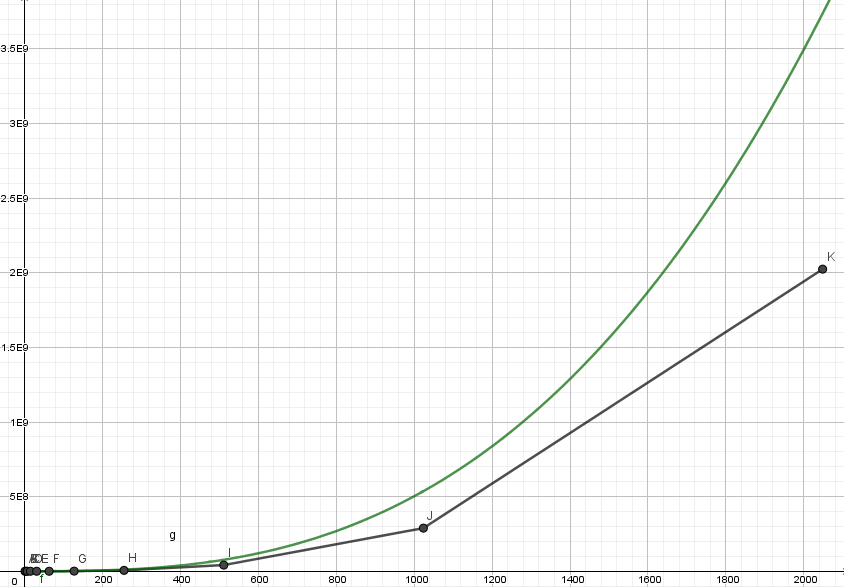
\includegraphics[width=100mm]{./imagenes/fig4.png}\\
		Figura 3: Resultados Strassen vs $n^{2.8}$
	\end{center}
	La grafica en color negro es la función f(n) que se propone, con base en los resultados obtenidos tras la implementacion del algoritmo, la grafica en color verde es  T(n)=${\theta(n^{2.8})}$, como observamos en la figura 3 la función representante del algoritmo de Strassen es muy similar a los resultados esperados, cabe aclarar que la variacion puede darse debido a que en la implementacion, se utilizaron unicamente matrices con orden ${2^{2}}$, por eso los saltos tan grandes entre el punto "j" y el punto "k", por lo que se concluye que cumple con los resultados esperados, por lo tanto, el tiempo computacional de la función Stressen es de tipo T(n)=${\theta(n^{2.8})}$.\\
	\newpage

	{\large ii)Para valores muy grandes de matrices compare el algoritmo de {\bf Strassen} con el producto usual de matrices (compara la complejidad).}\\
	
	\bigskip
	Para este inciso, crei conveniente primero realizar la comparacion del algoritmo de multiplicacion tradicional y la funcion obtenida en el salon de clases, y despues comparar los resultados de Strassen con la multiplicacion normal.
	
	\begin{center}
		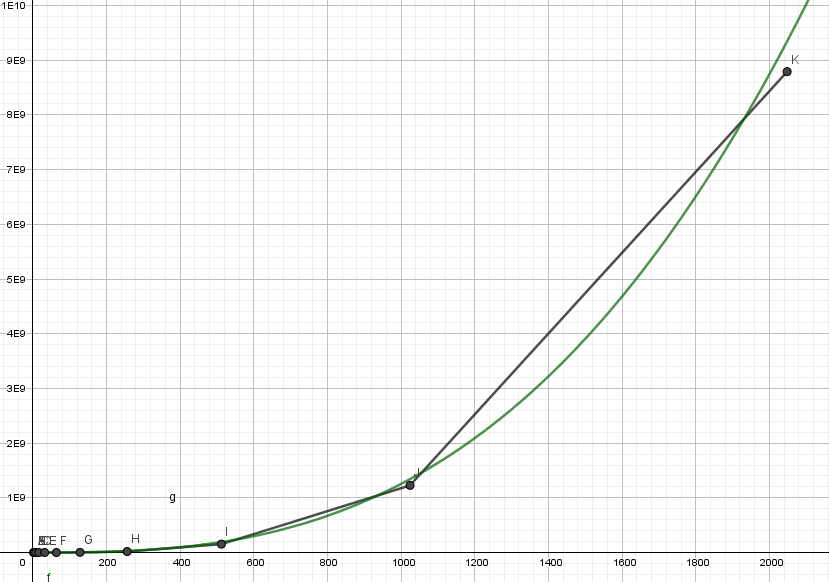
\includegraphics[width=100mm]{./imagenes/fig5.png}\\
		Figura 4: Resultados Multiplicacion Tradicional vs $n^{2.8}$
	\end{center}

	Como se puede observar en la figura 4, la grafica es de nuevo muy parecida, con los resultados obtenidos, se aprecia un cambio algo drastico en el salto del punto "J" al punto "K", esto se da, de igual manera que el caso anterior, a que las matrices utilizadas para este ejercicio son de orden ${2^{2}}$, sin embargo, por el comportamiento que se puede apreciar en el trayecto de la recta verde que representa a nuestra funcion propuesta, se nota que esta crece de mayor tamaño que la grafica de color negro, que representa los resultados obtenidos, de igual manera, la grafica propuesta se esta multiplicando por un excponente para aprecair mejor su comportamiento.
\newpage
	\begin{center}
		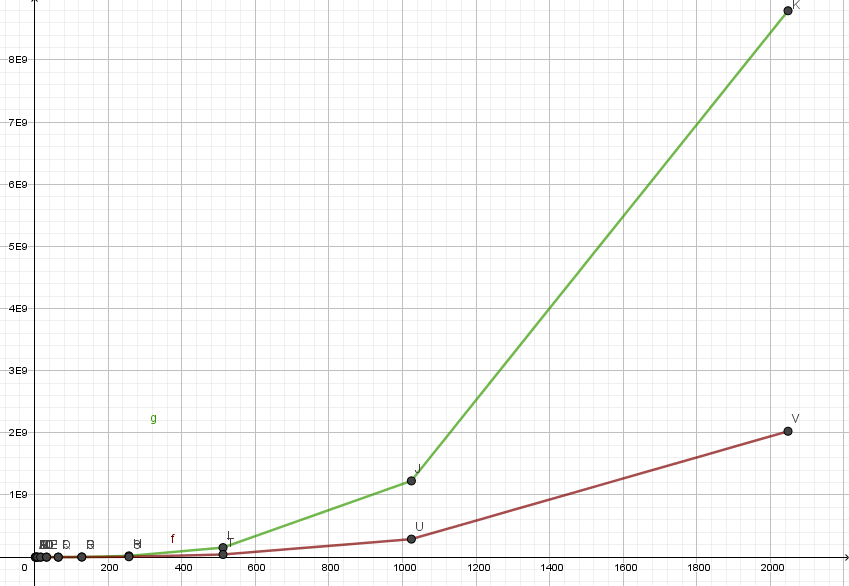
\includegraphics[width=100mm]{./imagenes/fig6.png}\\
		Figura 5: Resultados Multiplicacion Tradicional vs Strassen.
	\end{center}
	En la figura 5, podemos ver la comparacion de los resultados arrojados por strassen y los resultados arrojados por la multiplicacion tradicional. De color verde tenemos la funcion de Strassen, y de rojo la m.Tradicional.\\
	Podemos observar que la grafica representada por Strassen crece de manera mas rapida que la otra, sin embargo, esto es solamenter aplicable para matrices de tamaño muy grande, no se si este algoritmo sea el mas eficiente para esta multiplicacion, pero al momento de realizar operaciones tan grandes, sin duda alguna es de gran ayuda, al arrojar mejores resultados, podemos concluir que el algoritmo de Strassen es mas eficiente que el algoritmo tradicional, al momento de realizar multiplicaciones de matrices grandes.
	\newpage

	\section{Conclusi\'on}

	\bigskip
Esta practica fue muy entretenida, el analisis de algoritmos para determinar cual es mejor, es un tema que de verdad es muy fascinante, sin embargo, la realizacion de este algoritmo fue muy complicada, no pude realizarla en Python como lo venia haciendo, ya que Python no maneja matrices como tal, y el manejo de arreglo de arreglos es algo que aun me tiene con complicaciones, por lo que la realice en Java.\\
Regresando a la practica, el analisis de este algoritmo, mediante el metodo grafico fue sencillo, una vez completado, no conocia este algoritmo, y no se si sea el mejor, pero por ahora para la multiplicacion de matrices de gran tamaño, creo que es una opcion muy interesante.
	\bigskip

\end{document}